\documentclass[color, ddc]{tudscrreprt}
%\usepackage[T1]{fontenc}
% Achtung: LuaLaTeX!!
\usepackage[utf8]{luainputenc}
\usepackage[ngerman]{babel} 
\usepackage{underscore}
\shorthandoff{"}	

\usepackage{graphicx}
\usepackage{grffile}

\faculty{Fakultät Elektro- und Informationstechnik}
\chair{Institut für Automatisierungstechnik}
\begin{document}
    \title{Dokumentation Praktikum Mensch-Maschine-Systemtechnik}
    \author{Gruppe 2.3:
    Lukas Buntkiel, 
    Alexander Lehmann, 
    Miao Zhang, 
    Sven Schönfeld,
    Falk-Jonatan Strube}
    \maketitle

\tableofcontents

\chapter{Einleitung: Literatur \& Theoriebildung}

\section{Einordnung}

Hauptbestandteil der Aufgabenstellung ist das Entwerfen einer interaktiven Darstellung der Revisions-Struktur des Versionsverwaltungssystems (Version Control System, VCS) R43ples.

R43ples kann zur Versionsverwaltung von Named Graphs genutzt werden, dem Schlüs\-sel-Be\-stand\-teil des Semantic Web\cite{pascal:semanic-web}. Es verwendet dabei zur Verwaltung der Revisionen wiederum Named Graphs, in denen auch sämtliche, zur Darstellung der Struktur notwendigen, Informationen in Form von Linked Data enthalten sind \cite{graube:r43ples}. R43ples verwendet dabei ein ähnliches Konzept wie klassische Versionsverwaltungssysteme (wie z.B. git\cite{url:git-scm}) indem es Verzweigungen von Revisionen in Form von Branches sowie das Kennzeichnen spezieller Revisionen mit Tags unterstützt \cite{graube:r43ples}.

Der Hauptunterschied zu klassischen VCS liegt also weniger im Konzept der Versionsverwaltung selbst, als in der Anwendung dieses Konzeptes auf einen neuen Typ von Ressource (Named-Graphs). Es kann daher angenommen werden, dass durch andere VCS bereits Lösungen für die graphische Darstellung von Revisionen vorhanden sind, die im Verlauf dieser Arbeit analysiert werden können, um günstige Merkmale herauszuarbeiten.

\section{Theoriebildung}

VERARBEITUNG FOLIEN ERSTPRÄSENTATION
    
\chapter{Analyse}

\section{Analyse \& Entwurf}

DATEN IM turtle DIAGRAMM (LUKAS)
\subsection{Daten im turtle}
\def\arraystretch{1.5}
\begin{tabular}{l l c}
Bezeichnung & Nutzen & Kommentar\\
rdf:type & Gibt an, ob's Commit, Revision o. ä. & \\
delta Removed & & \\
delta Added & & \\
revisionNumber & & \\
revisionOf & & \\

\end{tabular}

\subsection{Darstellungen anderer Subversion Systeme}
\begin{itemize}
\item SVN \cite{url:svn-gource}
\item GIT \cite{url:git}
\item GIT \cite{url:gitready}
\end{itemize}

\subsection{Erster Entwurf}

\begin{figure}[ht!]
\centering
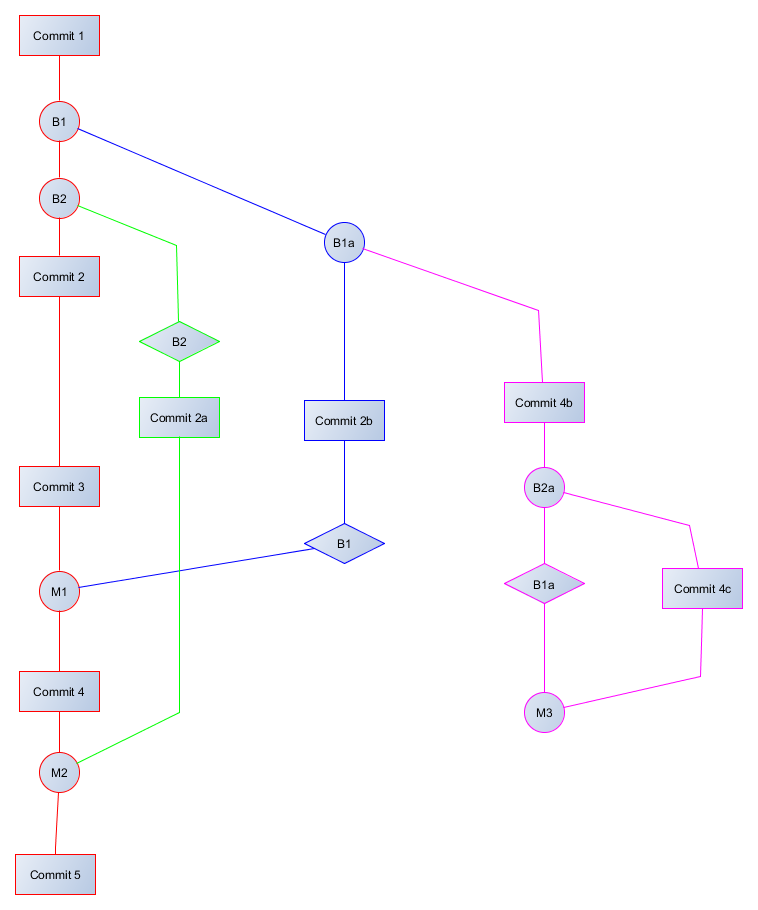
\includegraphics[width=90mm]{Skizzen/2014-12-12 VisualisierungsSkizze.png}
\caption{Erste Skizze}
\end{figure}

\chapter{Pflichtenheft}

\section{Produktfunktionen}
\subsection{Muss}
\begin{itemize}
\item Daten aus turtle-Datensatz auslesen (zum weiterverarbeiten)
\item Daten werden graphisch abgebildet
\end{itemize}

\subsection{Kann}
\begin{itemize}
\item Daten werden in in unterschiedlichen Darstellungsebenen dargestellt (Gesamt- und Detailübersicht)
\item Einzelansicht für die Details von Commits
\item Daten werden tabellarisch-strukturiert abgebildet
\end{itemize}

\subsection{Soll}
\begin{itemize}
\item Zweckmäßige Übergangsanimationen zwischen Darstellungsansichten
\end{itemize}

\section{Qualitätsanforderungen}
\begin{itemize}
\item Daten werden (aus den turtle-Datensätzen) unverfälscht abgebildet
\item Durch Informationsreduzierung (auf das nötigste) wird ein höhere Übersichtlichkeit erreicht (Minimierung der Darstellung von merges und commits durch Unterteilung in Detailansichten)
\end{itemize}

\section{Einschränkungen und Randbedingungen}
\begin{itemize}
\item Läuft auf neuerem Firefox und Chrome
\end{itemize}

\section{Annahmen und Abhängigkeiten}
\begin{itemize}
\item Nutzer ist mit r43ples und dem semantic web vertraut
\end{itemize}

\chapter{Gestaltungsentwurf}

\chapter{Abgabe}

\bibliographystyle{unsrt}
\bibliography{Literatur}

\end{document}